\documentclass[letterpaper,12pt,fleqn]{article}
\usepackage{matharticle}
\usepackage{siunitx}
\pagestyle{empty}

\begin{document}

\section*{Area}

There are some problems that algebra alone cannot solve:

\subsection*{Area Under a Curve}

\begin{definition}[Summation Problem]
  A \emph{summation problem} seeks to determine the total amount of a quantity based on its rate of change over
  a particular range of values (region) of the other quantity.
\end{definition}

For summation problems, a rate-of-change function \(f(x)\) and a region of the independent variable \(x\) are
given.

\begin{example}
  A car is traveling at a constant speed of \SI{60}{mph}.  How far does the car travel in \SI{2}{hours}?

  This is simply a distance equal rate times time problem:
  \[d=(\SI{60}{mi/hr})(\SI{2}{hr})=\SI{120}{mi}\]
  Interpreted geometrically:

  \bigskip

  \begin{center}
    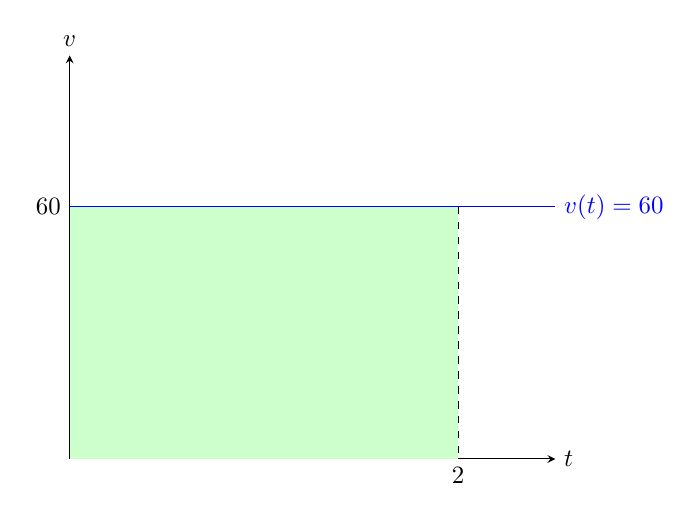
\begin{tikzpicture}[scale=0.9]
      \begin{axis}[
          axis lines=middle,
          xmin=0,
          xmax=5,
          ymin=0,
          ymax=8,
          ticks=none,
          xlabel={\(t\)},
          ylabel={\(v\)},
          x label style={at={(axis cs:5,0)},anchor=west},
          y label style={at={(axis cs:0,8)},anchor=south},
          clip=false
        ]
        \addplot [domain=0:5,blue] {5} node [right] {\(v(t)=60\)};
        \node [left] at (0,5) {\(60\)};
        \fill [green!20!white] (0,0) rectangle (4,5);
        \draw [dashed] (4,5) -- (4,0) node [below] {\(2\)};
      \end{axis}
    \end{tikzpicture}
  \end{center}

  \bigskip

  Note that the area under the rate-of-change curve in the selected region is calculated.
\end{example}

But what if the rate-of-change function is not constant?  The total is still the area under the curve.

\begin{example}
  A car is traveling with a speed that increases linearly from \SI{0}{mph} to \SI{60}{mph} after one hour, and then
  decreases linearly from \SI{60}{mph} to \SI{0}{mph} over the next hour.  How far does the car travel?

  \bigskip

  \begin{center}
    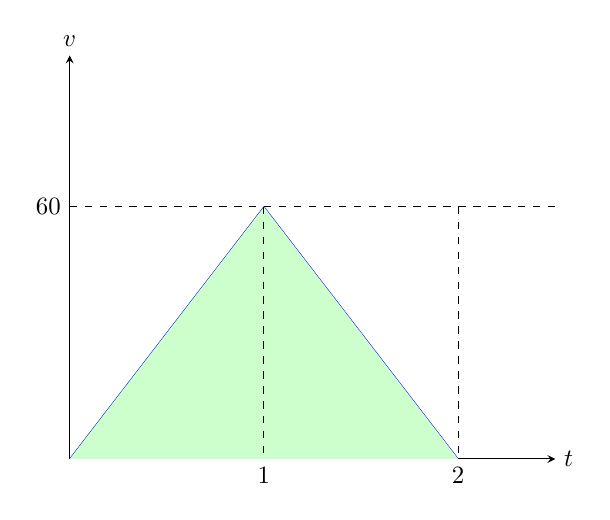
\begin{tikzpicture}[scale=0.9]
      \begin{axis}[
          axis lines=middle,
          xmin=0,
          xmax=5,
          ymin=0,
          ymax=8,
          ticks=none,
          xlabel={\(t\)},
          ylabel={\(v\)},
          x label style={at={(axis cs:5,0)},anchor=west},
          y label style={at={(axis cs:0,8)},anchor=south},
          clip=false
        ]
        \addplot [dashed,domain=0:5] {5};
        \addplot [domain=0:2,blue] {2.5*x};
        \addplot [domain=2:4,blue] {2.5*(4-x)};
        \node [left] at (0,5) {\(60\)};
        \fill [green!20!white] (0,0) -- (4,0) -- (2,5) -- cycle;
        \draw [dashed] (4,5) -- (4,0) node [below] {\(2\)};
        \draw [dashed] (2,5) -- (2,0) node [below] {\(1\)};
      \end{axis}
    \end{tikzpicture}
  \end{center}
  \[d=\frac{1}{2}(\SI{60}{mi/hr})(\SI{2}{hr})=\SI{60}{mi}\]
\end{example}

But what happens if there is no convenient geometric formula for the area under the curve?

\begin{center}
  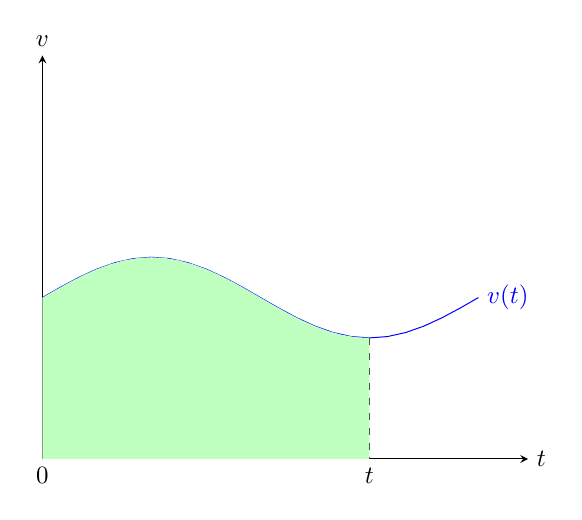
\begin{tikzpicture}[scale=0.9]
    \begin{axis}[
        axis lines=middle,
        xmin=0,
        xmax=7,
        ymin=0,
        ymax=5,
        ticks=none,
        xlabel={\(t\)},
        ylabel={\(v\)},
        x label style={at={(axis cs:7,0)},anchor=west},
        y label style={at={(axis cs:0,5)},anchor=south},
        clip=false
      ]
      \addplot [domain=0:2*pi,blue] {2+(1/2)*sin(deg(x))} node [right] {\(v(t)\)};
      \draw [dashed] (3*pi/2,3/2) -- (3*pi/2,0);
      \fill [green!25!white] (0,0) -- (0,2) --  plot [domain=0:3*pi/2] ({\x},{2+(1/2)*sin(deg(\x))}) --
      (3*pi/2,0) -- cycle;
      \node [below] at (0,0) {\(0\)};
      \node [below] at (3*pi/2,0) {\(t\)};
    \end{axis}
  \end{tikzpicture}
\end{center}

Unfortunately, there is no way using just algebra to determine the area under a general curve.

Why do we care?
\begin{enumerate}
\item How far does a car travel that varies its speed along the way?
\item How much product is produced during a chemical reaction that has a particular reaction rate?
\item What is the projected population given a particular growth rate?
\item Which requires less work to lift a box: pushing it up a ramp or lifting it with a pulley.
\end{enumerate}

\end{document}
